\documentclass[10pt, landscape]{article}
\usepackage[scaled=0.92]{helvet}
\usepackage{calc}
\usepackage{multicol}
\usepackage{ifthen}
\usepackage[a4paper,margin=3mm,landscape]{geometry}
\usepackage{amsmath,amsthm,amsfonts,amssymb}
\usepackage{color,graphicx,overpic}
\usepackage{hyperref}
\usepackage{newtxtext} 
\usepackage{enumitem}
\usepackage[table]{xcolor}
\usepackage{mathtools}
% for drawing diragrams/graphs
\usepackage{tikz}
\usetikzlibrary{arrows.meta}
\usetikzlibrary{calc}
\setlist{nosep}

% ADDITIONAL USEFUL PACKAGES:
% for matrices
\usepackage{nicematrix}
% for relations
\usepackage{cancel}
\usepackage{ mathrsfs }
% for including images
\graphicspath{ {./images/} }


\pdfinfo{
  /Title (CS2040S.pdf)
  /Creator (TeX)
  /Producer (pdfTeX 1.40.0)
  /Author (Jovyn)
  /Subject (CS2040S)
  /Keywords (CS2040S, nus,cheatsheet,pdf)}

% Turn off header and footer
\pagestyle{empty}

\newenvironment{tightcenter}{%
  \setlength\topsep{0pt}
  \setlength\parskip{0pt}
  \begin{center}
}{%
  \end{center}
}

% redefine section commands to use less space
\makeatletter
\renewcommand{\section}{\@startsection{section}{1}{0mm}%
                                {-1ex plus -.5ex minus -.2ex}%
                                {0.5ex plus .2ex}%x
                                {\normalfont\large\bfseries}}
\renewcommand{\subsection}{\@startsection{subsection}{2}{0mm}%
                                {-1explus -.5ex minus -.2ex}%
                                {0.5ex plus .2ex}%
                                {\normalfont\normalsize\bfseries}}
\renewcommand{\subsubsection}{\@startsection{subsubsection}{3}{0mm}%
                                {-1ex plus -.5ex minus -.2ex}%
                                {1ex plus .2ex}%
                                {\normalfont\small\bfseries}}%
\renewcommand{\familydefault}{\sfdefault}
\renewcommand\rmdefault{\sfdefault}
%  makes nested numbering (e.g. 1.1.1, 1.1.2, etc)
\renewcommand{\labelenumii}{\theenumii}
\renewcommand{\theenumii}{\theenumi.\arabic{enumii}.}
\renewcommand\labelitemii{•}
\renewcommand\labelitemiii{•}
%  convenient absolute value symbol
\newcommand{\abs}[1]{\vert #1 \vert}
%  convenient floor and ceiling
\newcommand{\floor}[1]{\lfloor #1 \rfloor}
\newcommand{\ceil}[1]{\lceil #1 \rceil}
%  convenient modulo
\newcommand{\Mod}[1]{\ \mathrm{mod}\ #1}
%  for logical not operator, iff symbol, convenient "if/then"
\renewcommand{\lnot}{\mathord{\sim}}
\let\then\rightarrow
\let\Then\Rightarrow
%  vectors
\newcommand{\vv}[1]{\boldsymbol{#1}}
\newcommand{\VV}[1]{\overrightarrow{#1}}
%  column vector
\newcommand{\cvv}[1]{\left(\begin{smallmatrix}#1\end{smallmatrix}\right)}
\newcommand{\code}[1]{\textcolor{myblue}{\texttt{#1}}}
\newcommand\bggreen{\cellcolor{green!10}}

\makeatother
\definecolor{myblue}{cmyk}{1,.72,0,.38}
\everymath\expandafter{\the\everymath \color{myblue}}
% Define BibTeX command
\def\BibTeX{{\rm B\kern-.05em{\sc i\kern-.025em b}\kern-.08em
    T\kern-.1667em\lower.7ex\hbox{E}\kern-.125emX}}

% Don't print section numbers
\setcounter{secnumdepth}{0}

\setlength{\parindent}{0pt}
\setlength{\parskip}{0pt plus 0.5ex}
%% this changes all items (enumerate and itemize)
\setlength{\leftmargini}{0.5cm}
\setlength{\leftmarginii}{0.4cm}
\setlength{\leftmarginiii}{0.5cm}
\setlist[itemize,1]{leftmargin=2mm,labelindent=1mm,labelsep=1mm}
\setlist[itemize,2]{leftmargin=3mm,labelindent=1mm,labelsep=1mm}
\setlist[itemize,3]{leftmargin=3mm,labelindent=1mm,labelsep=1mm}

%My Environments
\newtheorem{example}[section]{Example}
% -----------------------------------------------------------------------

\begin{document}
\raggedright
\footnotesize
\begin{multicols}{4
    '}


% multicol parameters
% These lengths are set only within the two main columns
\setlength{\columnseprule}{0.25pt}
\setlength{\premulticols}{1pt}
\setlength{\postmulticols}{1pt}
\setlength{\multicolsep}{1pt}
\setlength{\columnsep}{2pt}

\begin{center}
    \fbox{%
        \parbox{0.8\linewidth}{\centering \textcolor{black}{
            {\Large\textbf{CS2040S}}
            \\ \normalsize{AY20/21 sem 2}}
            \\ {\footnotesize \textcolor{myblue}{by jovyntls}}
        }%
    }
\end{center}

\section{ORDERS OF GROWTH}
\subsection{definitions}
\begin{center}
    $T(n) = O(f(n))$ 
    \\* if $\exists c, n_0 > 0$ such that for all $n > n_0$, $T(n) \leq cf(n)$
    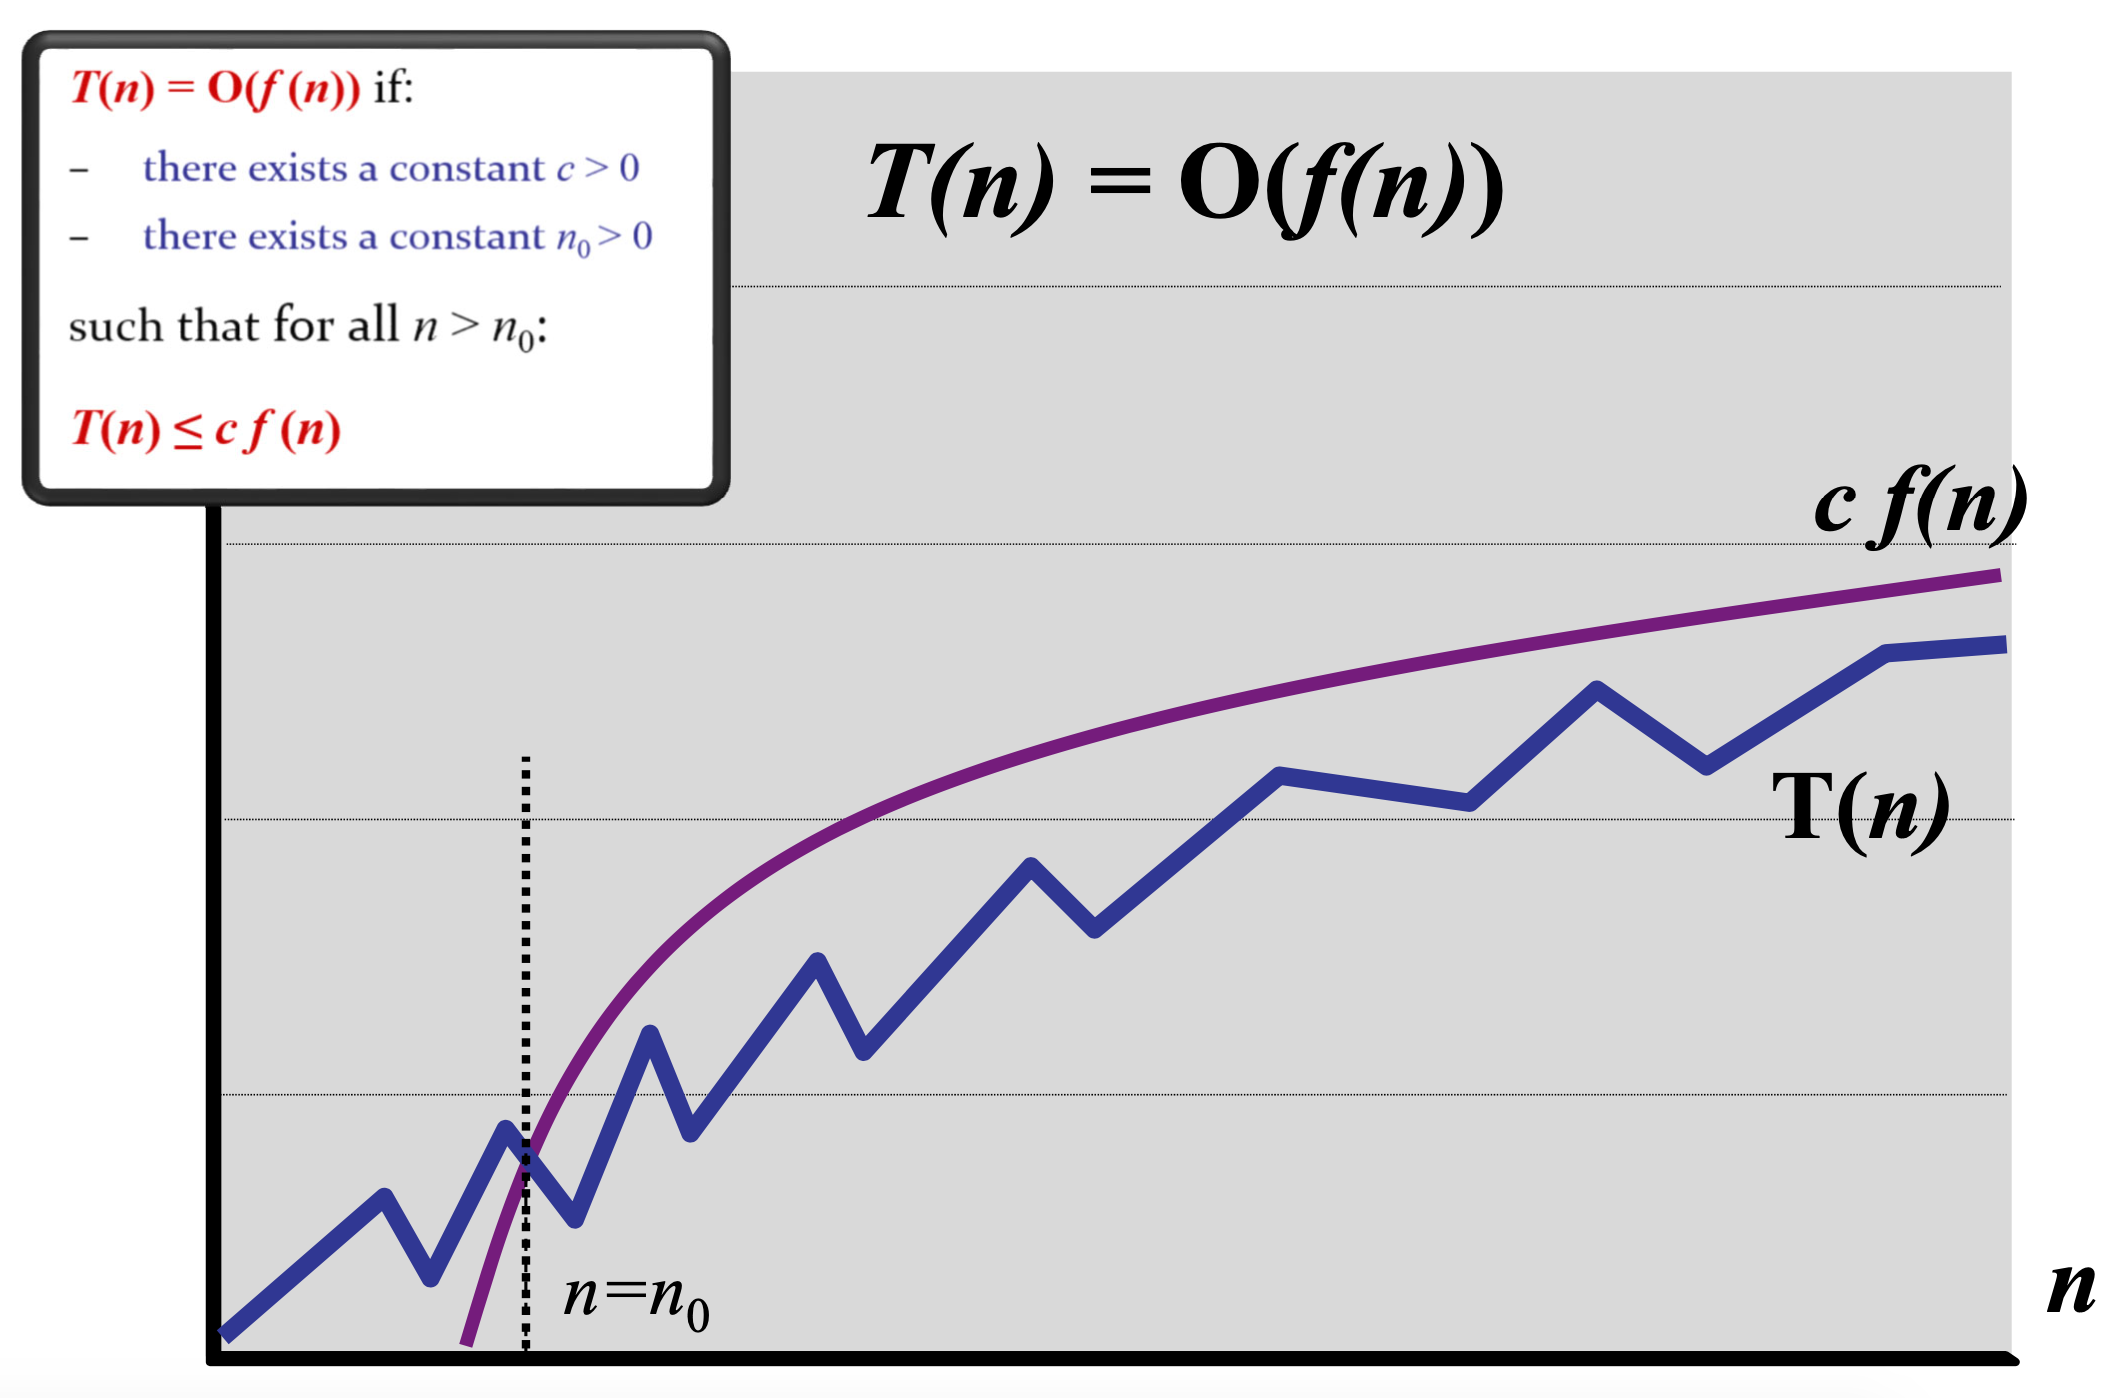
\includegraphics[width=0.6\linewidth]{cs2040s-big-o.png}
    
    $T(n) = \Omega(f(n))$
    \\* if $\exists c, n_0 > 0$ such that for all $n > n_0$, $T(n) \geq cf(n)$
    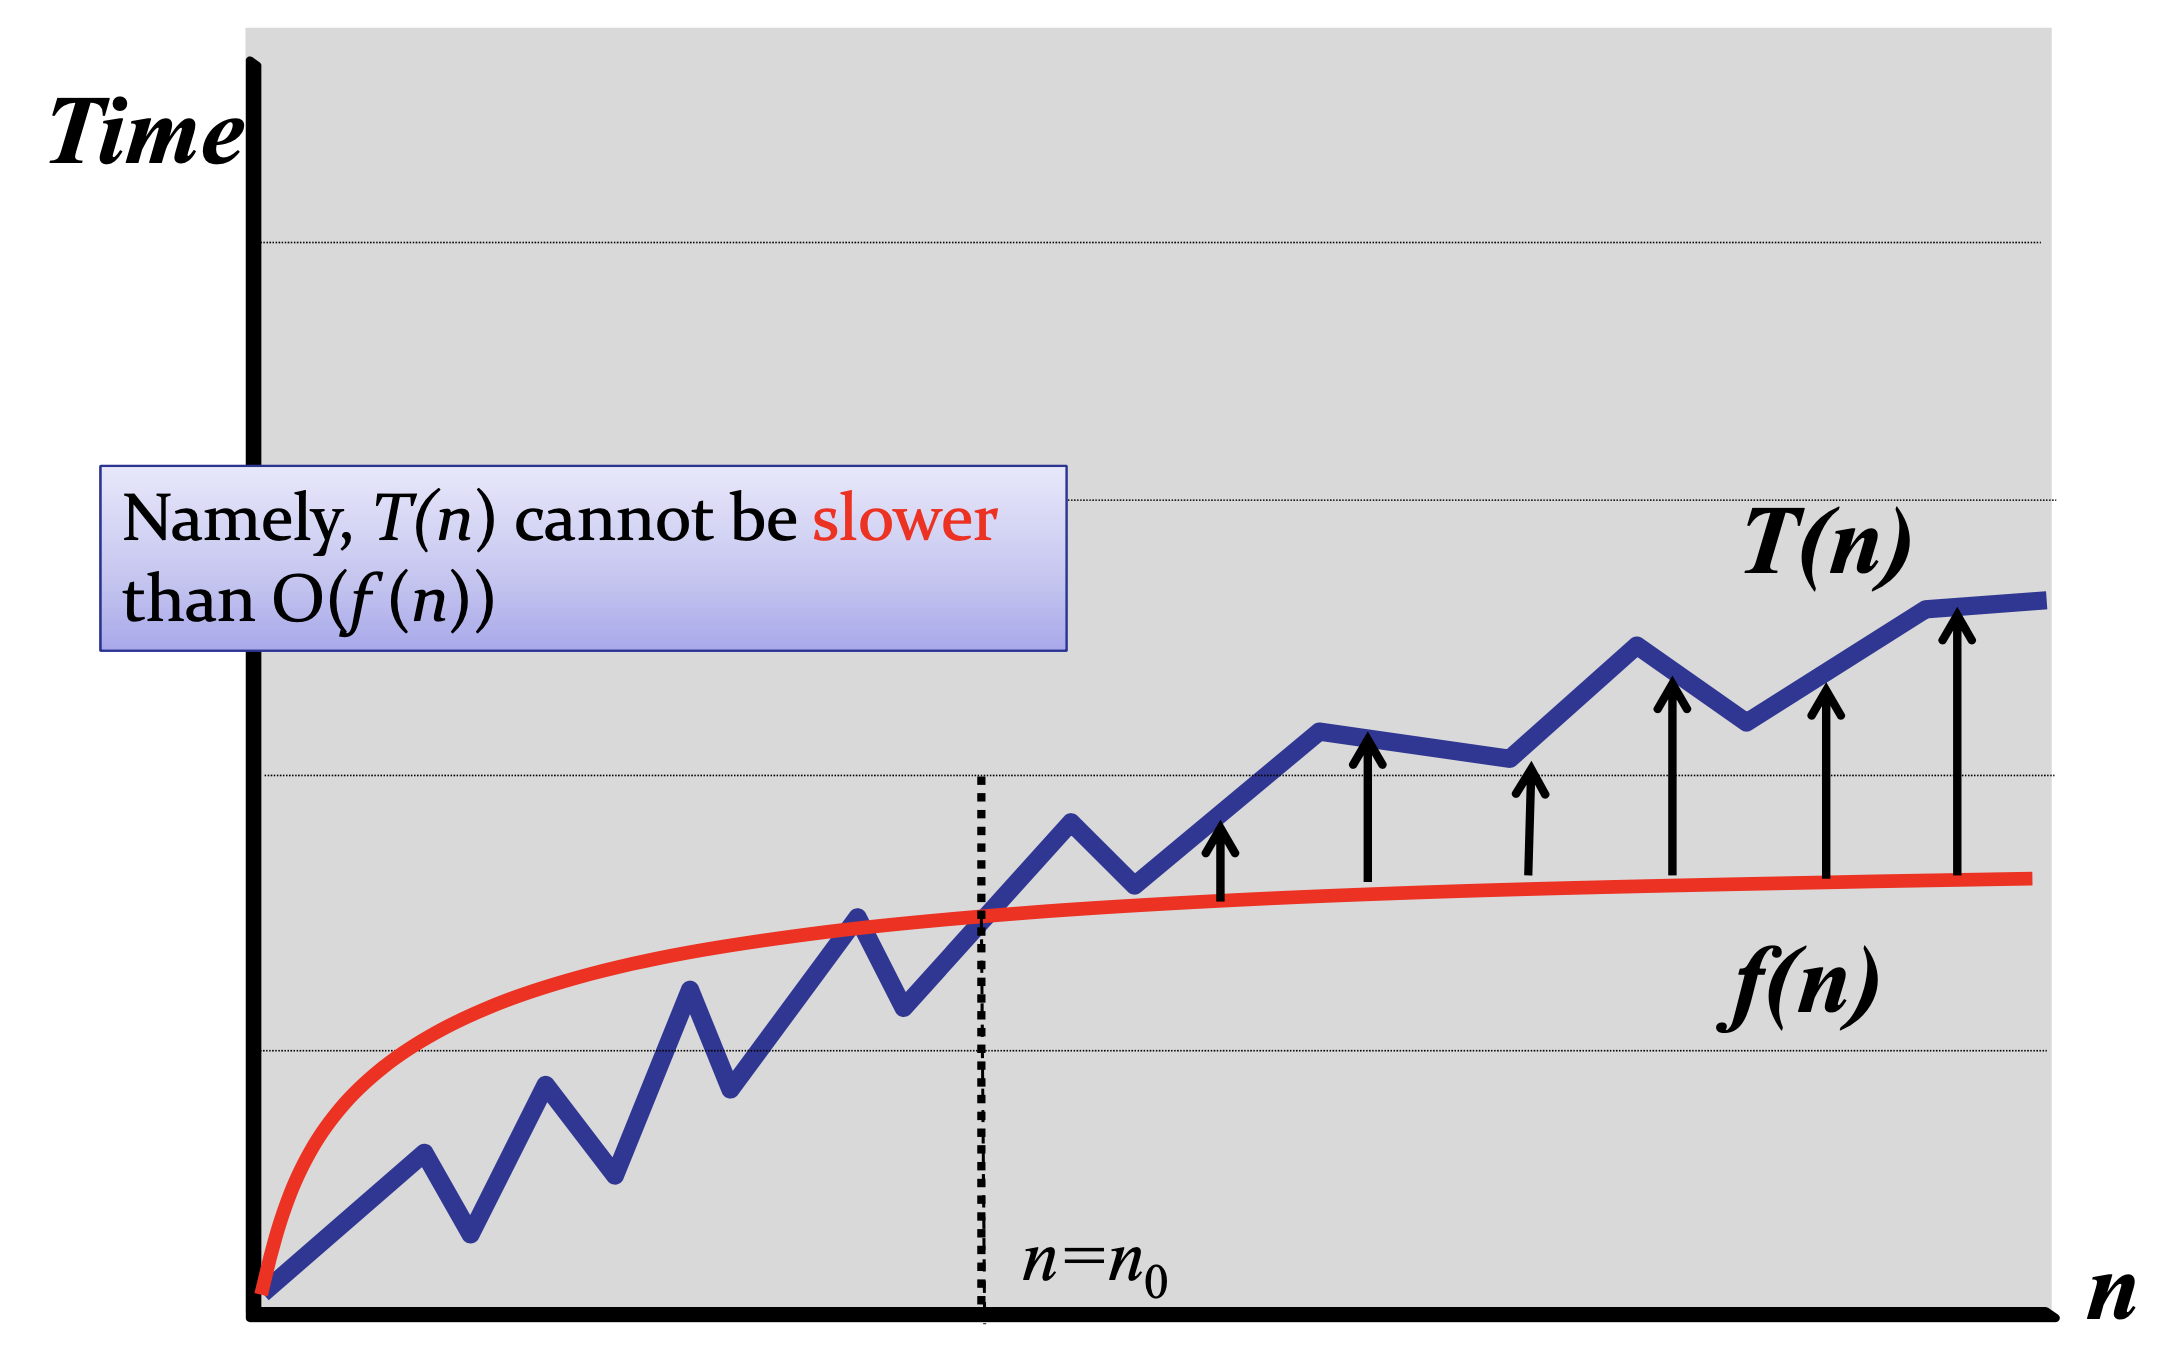
\includegraphics[width=0.6\linewidth]{cs2040s-big-omega.png}

    $T(n) = \Theta(f(n))$
    \\* $\iff T(n) = O(f(n))$ and $T(n) = \Omega(f(n))$
    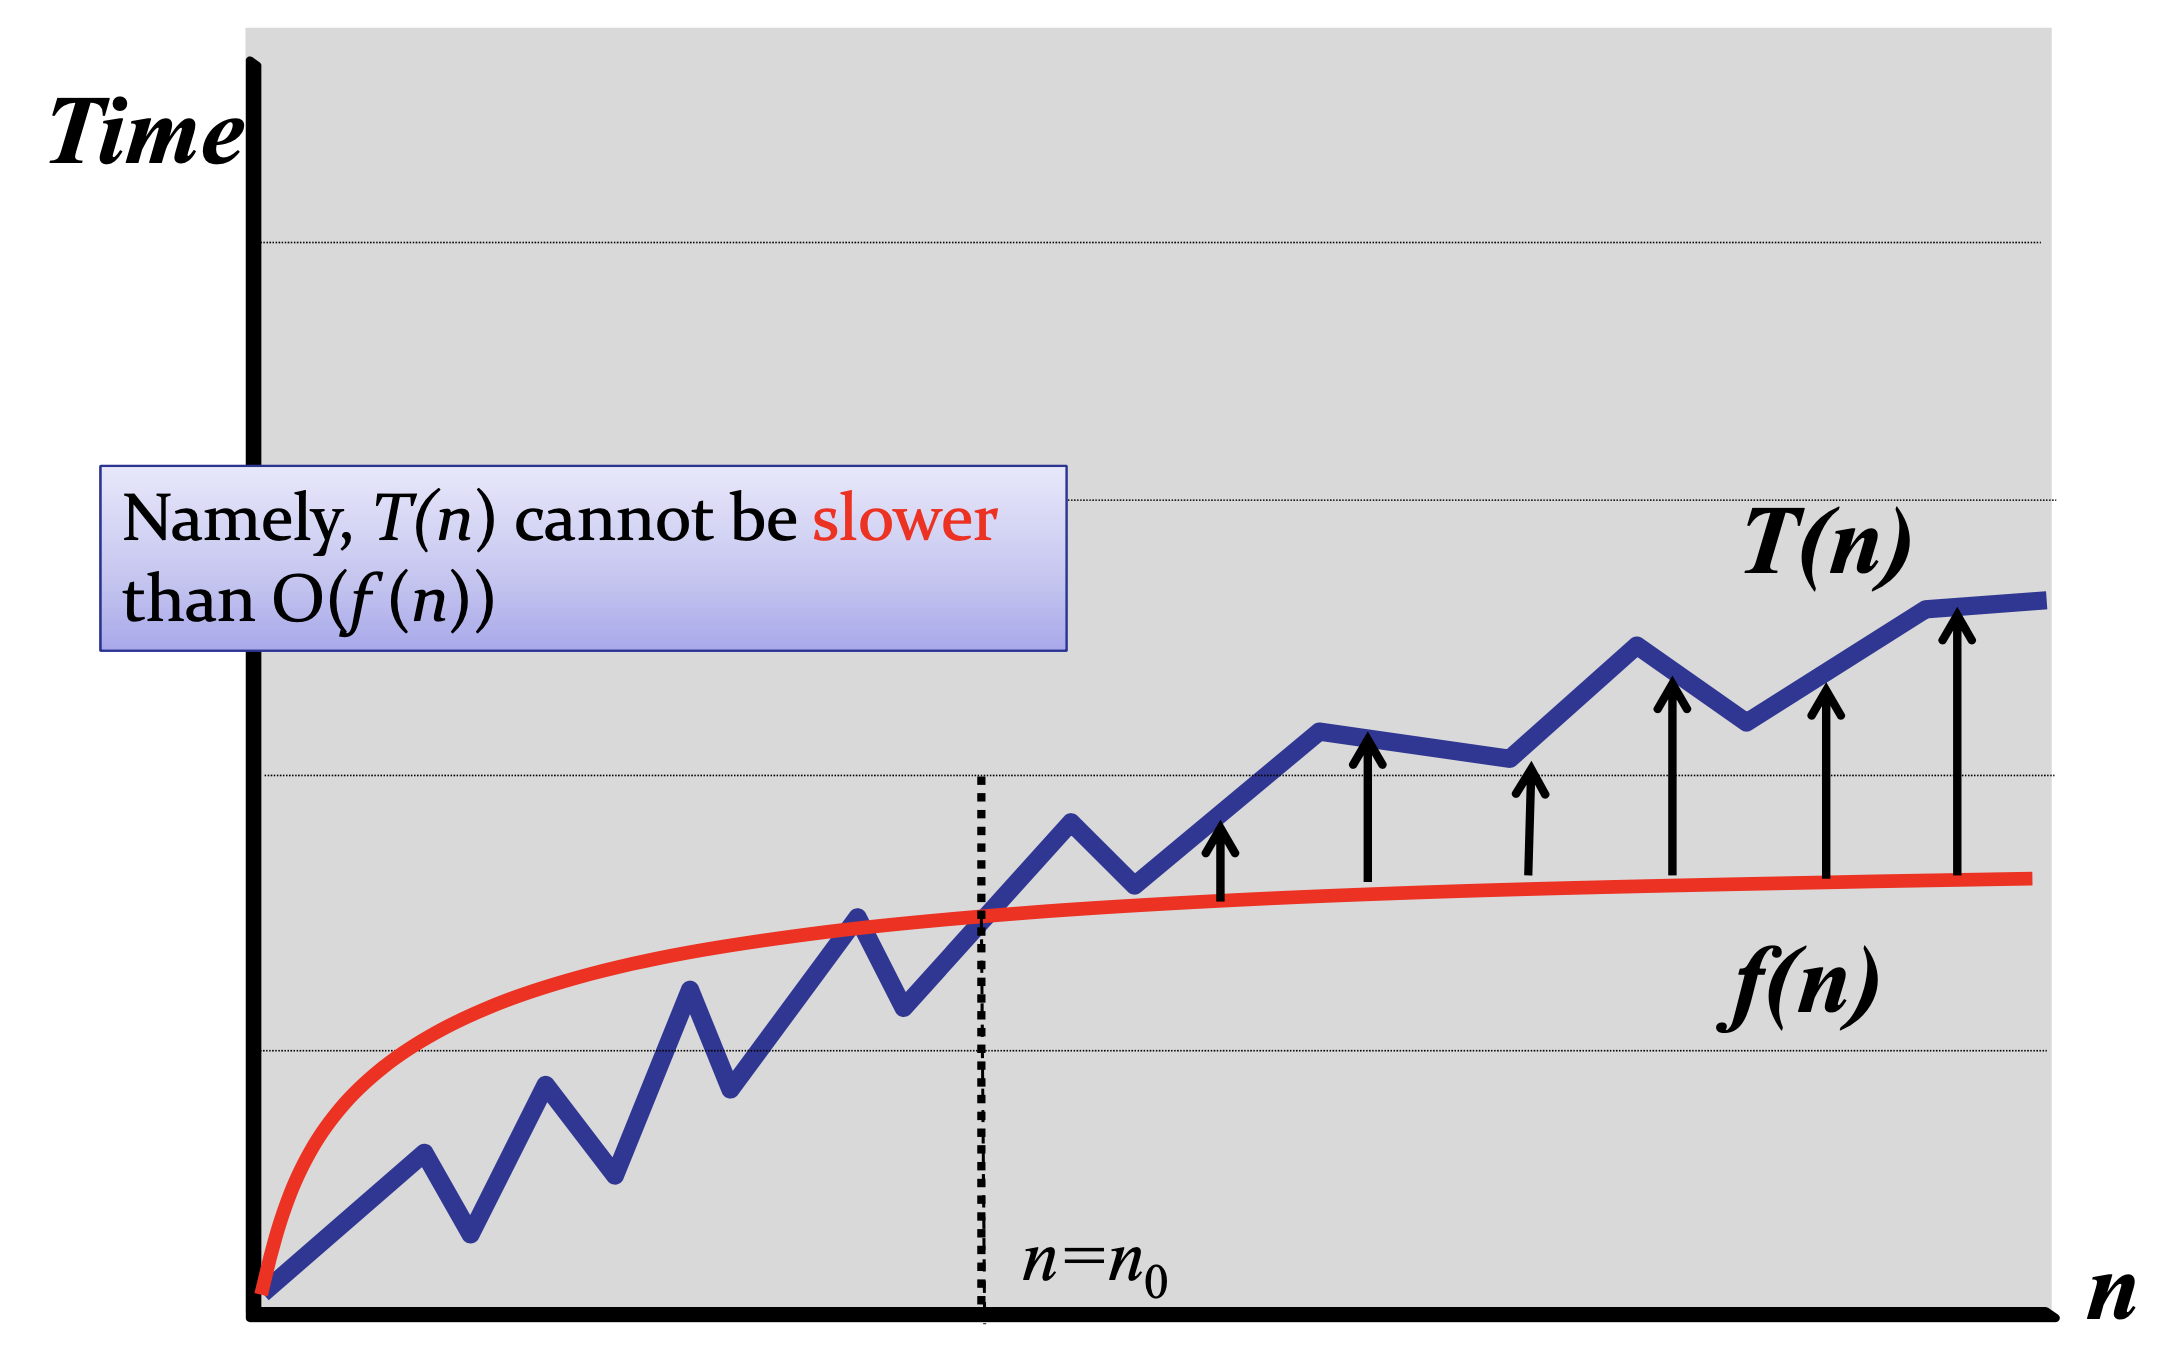
\includegraphics[width=0.6\linewidth]{cs2040s-big-omega.png}
\end{center}

\subsection{properties}
Let $T(n) = O(f(n))$ and $S(n) = O(g(n))$ 
\begin{itemize}
    \item addition: $T(n) + S(n) = O(f(n) + g(n))$
    \item multiplication: $T(n) * S(n) = O(f(n) * g(n))$
    \item composition: $f_1 \circ f_2 = O(g_1 \circ g_2)$
    \item if/else statements: $\text{cost} = \max(c1, c2) \leq c1+c2$
\end{itemize}

\subsubsection{notable}
\begin{itemize}
    \item $\sqrt{n}\log n$ is $O(n)$
    \item $O(2^{2n}) \neq O(2^n)$
    \item $O(\log (n!)) = O(n\log n)$
\end{itemize}

\section{SORTING}
\subsection{overview}
\textbf{Bubble Sort}
\begin{itemize}
    \item compare adjacent items and swap 
\end{itemize}

\textbf{Selection Sort}
\begin{itemize}
    \item takes the smallest element and swaps into place
    \item after $k$ iterations: the first $k$ elements are sorted 
\end{itemize}

\textbf{Insertion Sort}
\begin{itemize}
    \item from left to right: swap element leftwards until it's smaller than the next element. repeat for next element
    \item tends to be faster than the other $O(n^2)$ algorithms
\end{itemize}

\textbf{Merge Sort}
\begin{itemize}
    \item divide and conquer algorithm 
    \item mergeSort first half; mergeSort second half; merge
\end{itemize}

\textbf{Quick Sort}
\begin{itemize}
    \item partition algorithm: $O(n)$
    \begin{itemize}
        \item take first element as partition. 2 pointers from left to right
        \begin{itemize}
            \item left pointer moves until element > pivot
            \item right pointer moves until element < pivot
            \item swap elements until left = right. 
        \end{itemize}
        \item then swap partition and left=right index.
    \end{itemize}
\end{itemize}

\subsection{optimisations of QuickSort}
\begin{itemize}
    \item array of duplicates: $O(n^2)$ without 3-way partitioning
    \item stable if the partitioning algo is stable.
    \item extra memory allows quickSort to be stable.
\end{itemize}

\subsubsection{choice of pivot}
\begin{itemize}
    \item worst case time of $O(n^2)$
    \begin{itemize}
        \item first/last/middle element
    \end{itemize}
    \item worst case (expected) time of $O(n\log n)$:
    \begin{itemize}
        \item median/random element
        \item split by fractions: O(nlogn)
    \end{itemize}
    \item choose at random: runtime is a random variable
\end{itemize}

\subsection{quickSelect}
\begin{itemize}
    \item $O(n)$ - to find the $k^{\text{th}}$ smallest element
    \item after partitioning, the partition is always in the correct position
\end{itemize}

\section{TREES}
\subsection{binary search trees (BST)}
\begin{itemize}
    \item a BST is either empty, or a node pointing to 2 BSTs.
    \item tree balance depends on order of insertion
    \item balanced tree: $O(h) = O(\log n)$
\end{itemize}

\subsubsection{BST operations}
\begin{itemize}
    \item \code{height, h(v) = max(h(v.left), h(v.right))}
    \begin{itemize}
        \item leaf nodes: \code{h(v)} = 0 
    \end{itemize}
    \item modifying operations
    \begin{itemize}
        \item \code{search}, \code{insert} - $O(h)$
        \item \code{delete} - $O(h)$
        \begin{itemize}
            \item case 1: no children - remove the node
            \item case 2: 1 child - remove the node, connect parent to child
            \item case 3: 2 children - delete the successor; replace node with successor
        \end{itemize}
    \end{itemize}
    \item query operations
    \begin{itemize}
        \item \code{searchMin} - $O(h)$ - recurse into left subtree
        \item \code{searchMax} - $O(h)$ - recurse into right subtree
        \item \code{successor} - $O(h)$
        \begin{itemize}
            \item if node has a right subtree: \code{searchMin(v.right)}
            \item else: traverse upwards and return the first parent that contains the key in its left subtree
        \end{itemize}
    \end{itemize}
\end{itemize}
\begin{center}
    < successor code >
\end{center}

\subsection{traversal}
\begin{center}
    \begin{multicols}{3}
        \textit{pre-order DFS}
        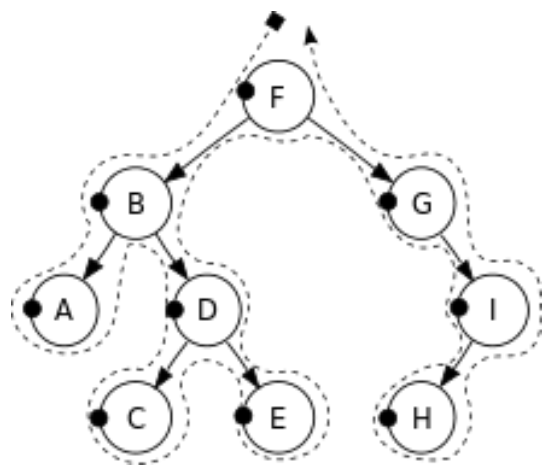
\includegraphics[width=0.9\linewidth]{../../CS1231S/images/cs1231s-ch11-preorder}
        \\* {\tiny\textbf{F-B-A-D-C-E-G-I-H}}
        
        \textit{in-order DFS}
        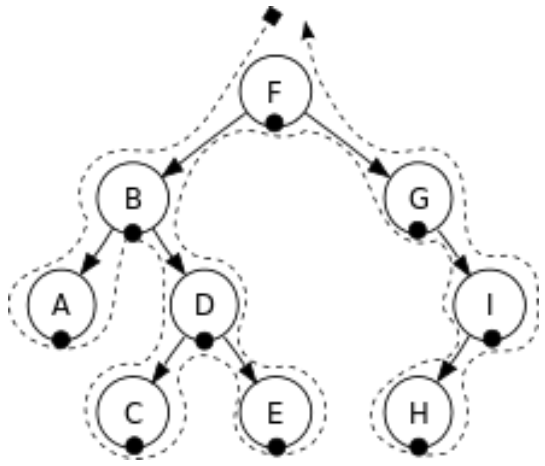
\includegraphics[width=0.9\linewidth]{../../CS1231S/images/cs1231s-ch11-inorder}
        \\* {\tiny\textbf{A-B-C-D-E-F-G-H-I}}
        
        \textit{post-order DFS}
        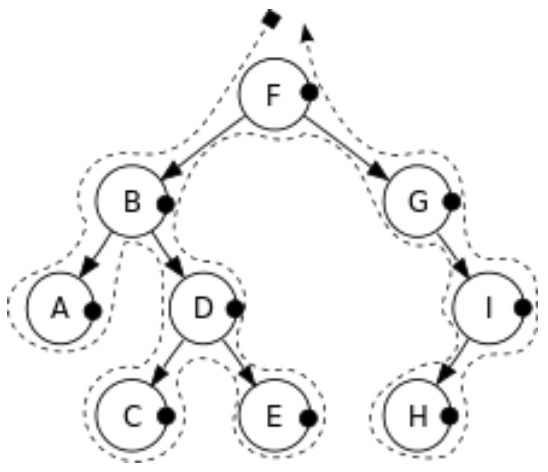
\includegraphics[width=0.9\linewidth]{../../CS1231S/images/cs1231s-ch11-postorder}
        \\* {\tiny\textbf{A-C-E-D-B-H-I-G-F}}
    \end{multicols}
\end{center}

\subsection{AVL Trees}
\begin{itemize}
    \item \textbf{height-balanced} 
    \begin{itemize}
        \item $\iff$ \code{|v.left.height - v.right.height| $\leq 1$}
    \end{itemize}
    \item each node is augmented with its height - \code{v.height = h(v)}
\end{itemize}

\subsubsection{rebalancing}
\begin{itemize}
    \item insertion: max. 2 rotations
    \item deletion: recurse all the way up
    \item rotations can create every possible tree shape.
\end{itemize}
[case 1] B is  \textbf{balanced: right-rotate}
\begin{center}
    $h(L) = h(M), \quad h(R) = h(M) - 1$
    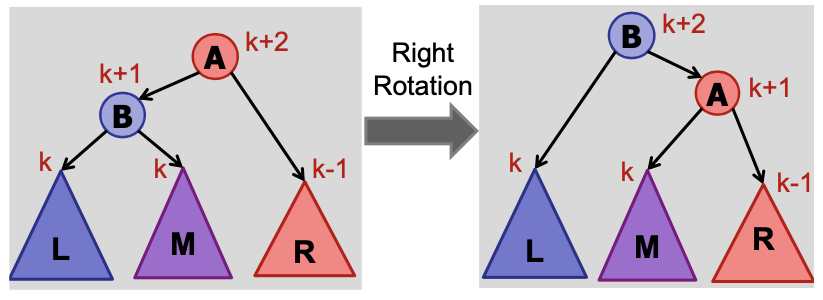
\includegraphics[width=0.8\linewidth]{cs2040s-rebalance-case-1.png}
\end{center}

[case 2] B is  \textbf{left-heavy: right-rotate}
\begin{center}
    $h(L) = h(M) + 1, \quad h(R) = h(M)$
    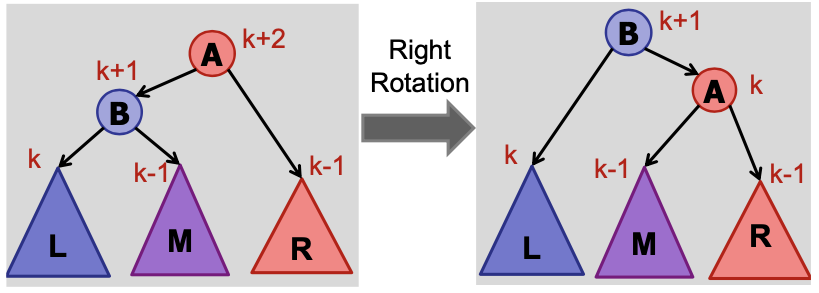
\includegraphics[width=0.8\linewidth]{cs2040s-rebalance-case-2.png}
\end{center}

[case 3] B is  \textbf{right-heavy: left-rotate(v.left), right-rotate(v)}
\begin{center}
    $h(L) = h(M) - 1, \quad h(R) = h(L)$
    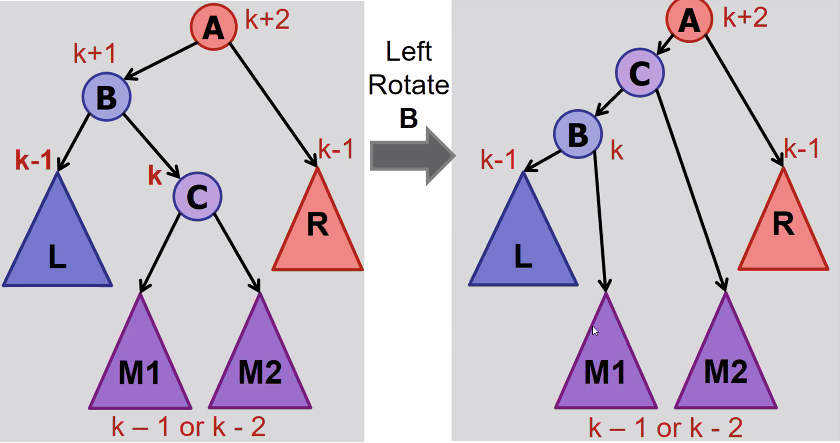
\includegraphics[width=0.8\linewidth]{cs2040s-rebalance-case-3-1.png}
    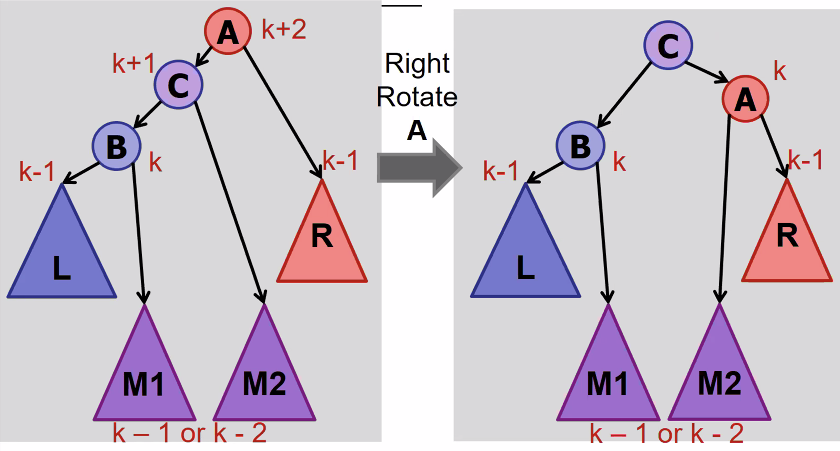
\includegraphics[width=0.8\linewidth]{cs2040s-rebalance-case-3-2.png}
\end{center}

\subsection{updating nodes after rotation}
\begin{center}
    weights
    \\* 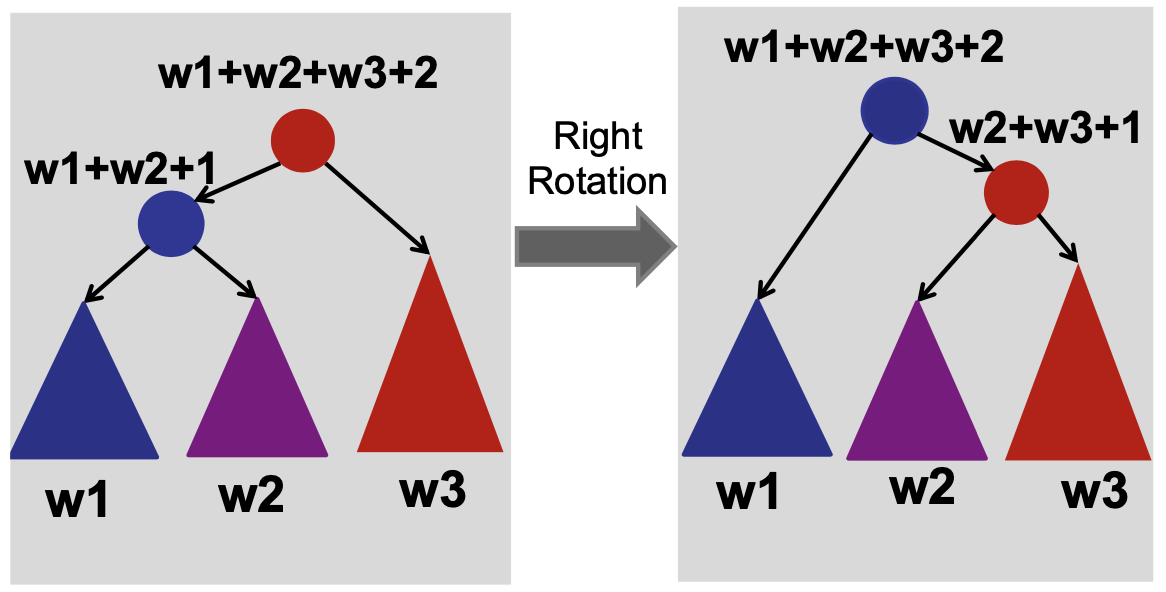
\includegraphics[width=0.8\linewidth]{cs2040s-rotate-weights.png}
    
    max
    \\* 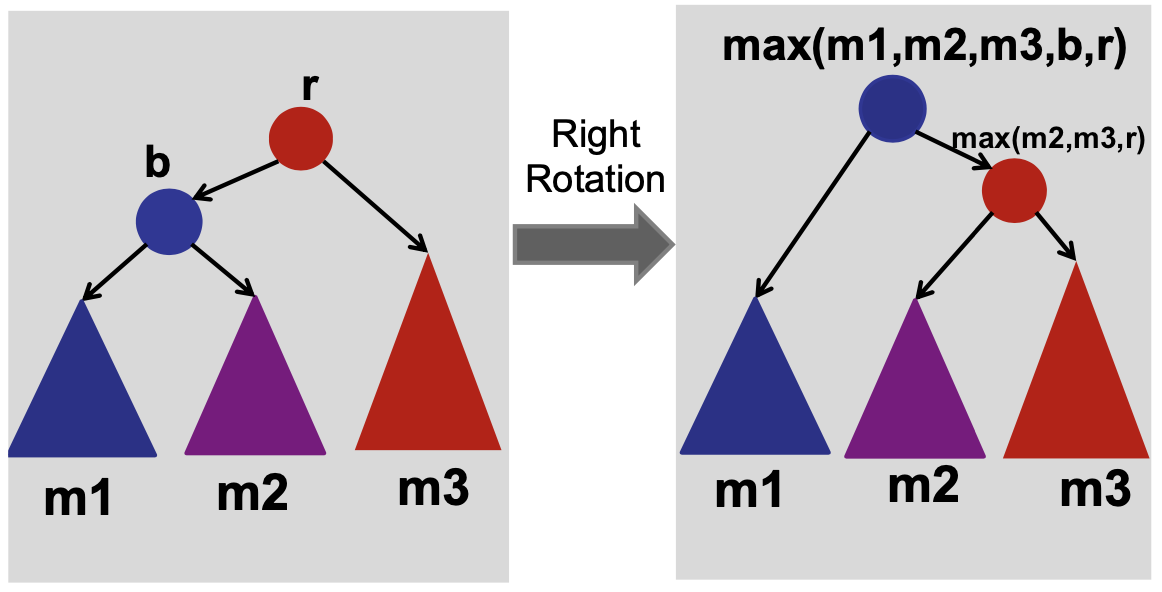
\includegraphics[width=0.8\linewidth]{cs2040s-rotate-max.png}
\end{center}

\subsection{Trie}
\begin{itemize}
    \item \code{search, insert} - $O(L)$ (for string of length $L$)
    \item space: $O($size of text $\cdot$ overhead$)$
\end{itemize}
\begin{center}
    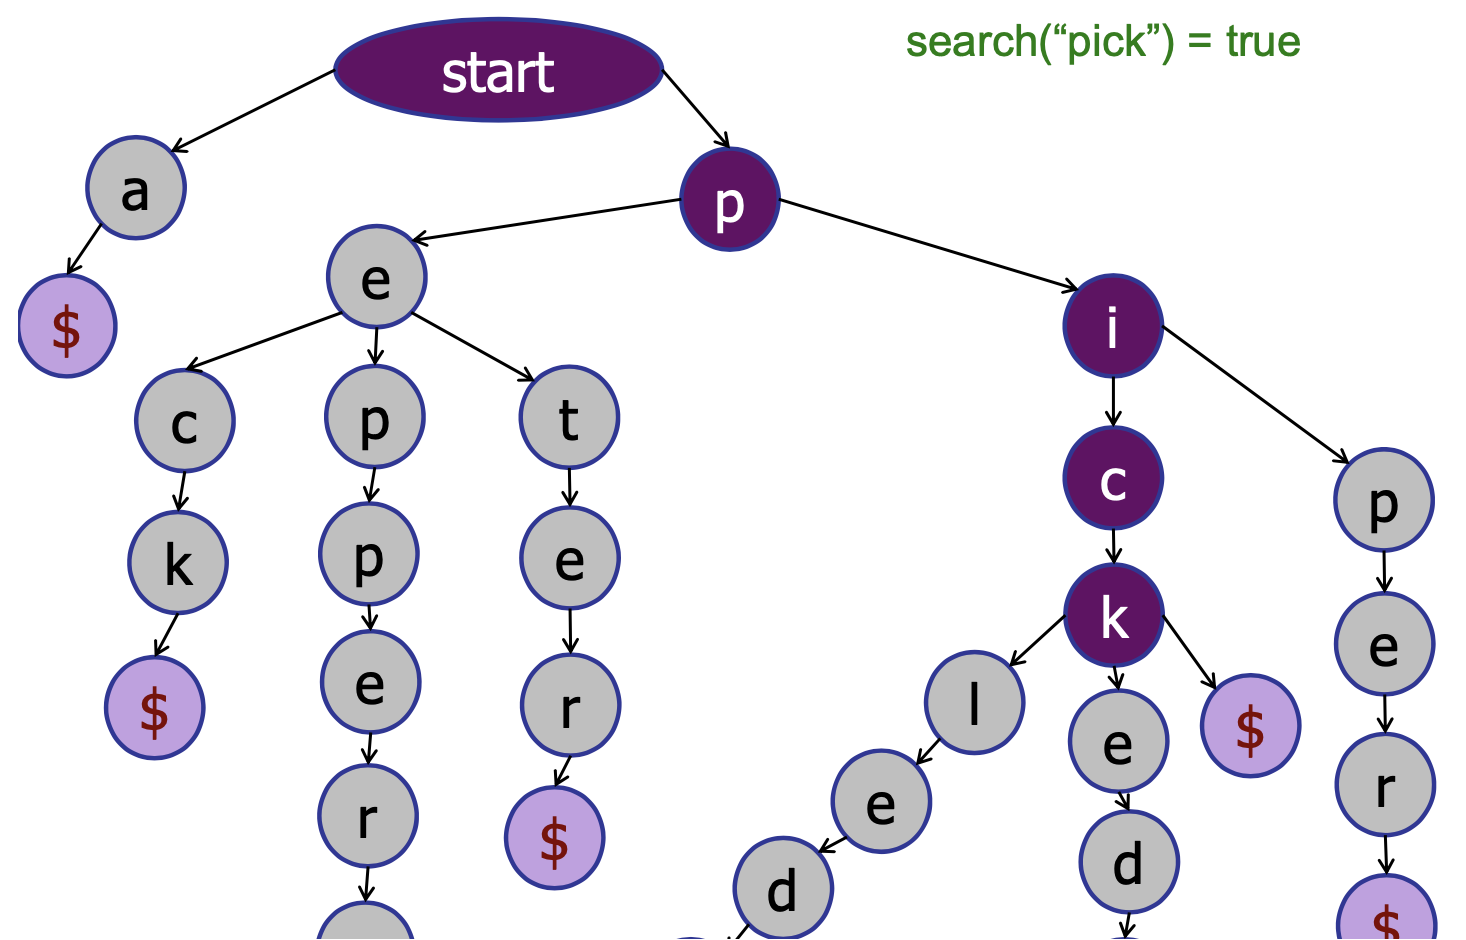
\includegraphics[width=0.8\linewidth]{cs2040s-trie.png}
\end{center}

\section{HASH TABLES}
\begin{itemize}
    \item very fast - faster than BST
    \item disadvantage: no successor/predecessor operation
\end{itemize}

\subsection{hashing}
Let the $m$ be the table size; 
let $n$ be the number of items;
let $cost(h)$ be the cost of the hash function

\begin{itemize}
    \item $load(\text{hash table})$, $\alpha = \frac{n}{m}$ 
    \begin{itemize}
        \item = average number of items per bucket
        \item = expected number of items per bucket 
    \end{itemize}
\end{itemize}

\subsubsection{hashing assumptions}
\begin{itemize}
    \item \textbf{simple uniform hashing assumption} 
    \begin{itemize}
        \item every key has an equal probability of being mapped to every bucket
        \item keys are mapped independently
    \end{itemize}
    \item \textbf{uniform hashing assumption} 
    \begin{itemize}
        \item every key is equally likely to be mapped to every permutation, independent of every other key.
        \item NOT fulfilled by linear probing
    \end{itemize}
\end{itemize}

\subsubsection{properties of a good hash function}
\begin{enumerate}
    \item able to enumerate all possible buckets - $h:U \to \{1..m\}$
    \begin{itemize}
        \item for every bucket $j$, $\exists i$ such that $h(key, i) = j$
    \end{itemize}
    \item simple uniform hashing assumption
\end{enumerate}

\subsection{hashCode}
\textbf{rules for the \code{hashCode()} method}
\begin{enumerate}
    \item always returns the same value, if the object hasn't changed
    \item if two objects are equal, they return the same hashCode
\end{enumerate}

\textbf{rules for the \code{equals} method}
\begin{itemize}
    \item reflexive - \code{x.equals(x) => true}
    \item symmetric - \code{x.equals(y)} $\Then$ \code{y.equals(x)}
    \item transitive - \code{x.equals(y), y.equals(z)} $\Then$ \code{x.equals(z)}
    \item consistent - always returns the same answer
    \item null is null - \code{x.equals(null) => false}
\end{itemize}

\subsection{chaining}
\begin{itemize}
    \item time complexity
    \begin{itemize}
        \item \code{insert(key, value)} - $O(1 + cost(h)) \Then O(1)$
        \begin{itemize}
            \item for $n$ items: expected maximum cost 
            \begin{itemize}
                \item $= O(\log n)$
                \item $= \Theta(\frac{\log n}{\log(\log(n))})$
            \end{itemize}
        \end{itemize}
        \item \code{search(key)} 
        \begin{itemize}
            \item worst case: $O(n + cost(h)) \Then O(n)$
            \item expected case: $O(\frac{n}{m} + cost(h)) \Then O(1)$
        \end{itemize}
    \end{itemize}
    \item total space: $O(m + n)$
\end{itemize}

\subsection{open addressing - linear probing}
\begin{itemize}
    \item redefined hash function: $h(k, i) = h(k, 1) + i \Mod{m}$
    \item \code{delete(key)}
    \begin{itemize}
        \item use a \textbf{tombstone value} - DON'T set to \code{null}
    \end{itemize}
    \item \textbf{performance}
    \begin{itemize}
        \item if the table is $\frac{1}{4}$ full, then there will be clusters of size $\Theta(\log n)$
        \item expected cost of an operation, $E[\# probes] \leq \frac{1}{1 - \alpha}$
            \\* (assume $\alpha < 1$ and uniform hashing)
    \end{itemize}
    \item \textbf{advantages}
    \begin{itemize}
        \item saves space (use empty slots vs linked list)
        \item better cache performance (table is one place in memory)
        \item rarely allocate memory (no new list-node allocation)
    \end{itemize}
    \item \textbf{disadvantages}
    \begin{itemize}
        \item more sensitive to choice of hash function (clustering)
        \item more sensitive to load (as $\alpha \to 1$, performance degrades)
    \end{itemize}
\end{itemize}

\subsubsection{double hashing}
\begin{center}
    for 2 functions $f, g$, define
    \\* $h(k, i) = f(k) + i \cdot g(k) \Mod m$
\end{center}
\begin{itemize}
    \item if $g(k)$ is relatively prime to $m$, then $h(k, i)$ hits all buckets
    \begin{itemize}
        \item e.g. for $g(k) = n^k$, $n$ and $m$ should be coprime.
    \end{itemize}
\end{itemize}

\subsection{table size}
assume chaining \& simple uniform hashing
\\* let $m_1 =$ size of the old hash table; 
$m_2 =$ size of the new hash table;
$n =$ number of elements in the hash table
\begin{itemize}
    \item growing the table: $O(m_1 + m_2 + n)$ 
    \item rate of growth
        \begin{tabular}{| c | c | c |}\hline
            \textbf{table growth} & \textbf{resize} & \textbf{insert $n$ items}\\\hline
            \text{increment by 1} & $O(n)$ & $O(n^2)$ \\\hline
            \text{double} & $O(n)$ & $O(n)$, average $O(1)$ \\\hline
            \text{square} & $O(n^2)$ & $O(n)$ \\\hline
        \end{tabular}
\end{itemize}



\section{PROBABILITY THEORY}
\begin{itemize}
    \item if an event occurs with probability $p$, the expected number of iterations needed for this event to occur is $\frac{1}{p}$.
    \item for \textbf{random variables}: expectation is always equal to the probability
    \item \textbf{linearity of expectation}: $E[A = B] = E[A] + E[B]$
\end{itemize}


\end{multicols}


\hrulefill \\
% \dotfill

\begin{multicols}{3}
    \begin{center}
        sorting
        \\* $
        \begin{array}{| c | c | c | c | c | c |}
            \hline\textbf{sort} & \textbf{best} & \textbf{average} & \textbf{worst} & \textbf{stable?} & \textbf{memory}
    
            \\\hline\text{bubble} & \Omega(n) & O(n^2) & O(n^2) & \checkmark & O(1)
            
            \\\hline\text{selection} & \Omega(n^2) & O(n^2) & O(n^2) & \times & O(1)
            
            \\\hline\text{insertion} & \Omega(n) & O(n^2) & O(n^2) & \checkmark & O(1)
            
            \\\hline\text{merge} & \Omega(n\log n) & O(n\log n) & O(n\log n) & \checkmark & O(n)
            
            \\\hline\text{quick} & \Omega(n\log n) & O(n\log n) & O(n^2) & \times & ?
            \\\hline
        \end{array} 
        $\

        sorting invariants
        \\*
        \begin{tabular}{| c | c |}
            \hline\textbf{sort} & \textbf{invariant} (after $k$ iterations)
            \\\hline bubble & largest $k$ elements are sorted
            \\\hline selection & smallest $k$ elements are sorted
            \\\hline insertion & first $k$ elements are in order
            \\\hline merge & –
            \\\hline quick & partition is in the right position
            \\\hline
        \end{tabular} 
        

        searching
        \\* \begin{tabular}{| c | c |}\hline
            \textbf{search} & \textbf{average} \\\hline
            \text{linear} & $O(n)$ \\\hline
            \text{binary} & $O(\log n)$ \\\hline
            \text{quickSelect} & $O(n)$ \\\hline
        \end{tabular}
        
        data structures (search/insert)
        \\* \begin{tabular}{| c | c | c |}\hline
            \textbf{data structure} & \textbf{search} & \textbf{insert}\\\hline
            \text{sorted array} & $O(\log n)$ & $O(n)$ \\\hline
            \text{unsorted array} & $O(n)$ & $O(1)$ \\\hline
            \text{linked list} & $O(n)$ & $O(1)$ \\\hline
            \text{tree} & $O(\log n)$ or $O(h)$ & $O(\log n)$ or $O(h)$ \\\hline
            \text{dictionary} & $O(\log n)$ & $O(\log n)$ \\\hline
            \text{symbol table} & $O(1)$ & $O(1)$ \\\hline
            \text{chaining} & $O(n + cost(h))$ & $O(1 + cost(h))$ \\\hline
            \text{open addressing} & $O(1)$ & $O(1)$ \\\hline
        \end{tabular}
    
    \end{center}
\end{multicols}

\begin{center}
\end{center}

\end{document}